\chapter{Additional material on Solar DM}

\section{Gravitational capture of DM by the Sun}
\label{sec:dm_analysis_capture_rates}

In this work I consider three possible scenarios for the \gls{dm} interactions: \gls{dm} scattering off electrons, spin-dependent (\gls{sd}) and spin-independent (\gls{si}) interactions with nuclei. For these last two, the cross sections will be given in terms of the \gls{sd} and \gls{si} elastic scattering \gls{dm} cross section off protons (assuming that the \gls{dm} interactions with protons and neutrons are identical), $\sigma_{p}^{\mathrm{SD}}$ and $\sigma_{p}^{\mathrm{SI}}$, as \cite{Bernal2012,Palomares2017}:
\begin{align}\label{2.3-2.4}
	\sigma_{i}^{\mathrm{SD}} &= \left(\frac{\tilde{\mu}_{A_{i}}}{\tilde{\mu}_{p}}\right)^{2} \frac{4(J_{i}+1)}{3 J_{i}} |\expval{S_{p,i}} + \expval{S_{n,i}}|^{2} \sigma_{p}^{\mathrm{SD}},\\
	\sigma_{i}^{\mathrm{SI}} &= \left(\frac{\tilde{\mu}_{A_{i}}}{\tilde{\mu}_{p}}\right)^{2} A_{i}^{2} \sigma_{p}^{\mathrm{SI}},
\end{align}
where $\tilde{\mu}_{A_{i}}$ is the reduced mass of the \gls{dm}-nucleus $i$ system, $\tilde{\mu}_{p}$ is the reduced mass of the \gls{dm}-proton system, $A_{i}$ and $J_{i}$ the mass number and total angular momentum of nucleus $i$, and $\expval{S_{p,i}}$ and $\expval{S_{n,i}}$ the expectation value of the spins of protons and neutrons averaged over all nucleons, respectively (see Ref. \cite{Bednyakov2004} for a review on spin expectation values).

Since the Sun is mainly composed of hydrogen, the capture of \gls{dm} from the halo is expected to occur mainly through \gls{sd} scattering. However, since the \gls{si} cross section is proportional to the square of the atomic mass, heavy elements can contribute to the capture rate (even though they constitute less than $2\%$ of the mass of the Sun). Heavy elements can also contribute to the \gls{sd} cross section if the \gls{dm} also has momentum-dependent interactions \cite{Catena2015}.

\gls{dm} particles can get captured by the Sun if after repeated scatterings off solar targets their final velocity is lower than the escape velocity of the Sun. In the limit of weak cross sections, this capture rate can be approximately written as \cite{Gould1987}:
\begin{equation}\label{2.5}
	C_{\odot}^{\mathrm{weak}} = \sum_{i} \int_{0}^{R_{\odot}} \mathrm{d}r \ 4\pi r^{2} \int_{0}^{\infty} \mathrm{d}u_{\chi} \ \frac{\rho_{\chi}}{m_{\chi}} \frac{f_{v_{\odot}}(u_{\chi})}{u_{\chi}} \omega(r) \int_{0}^{v_{e}(r)} \mathrm{d}v \ R_{i}^{-}(\omega \rightarrow v) |F_{i}(q)|^{2},
\end{equation}
where the summation extends over all possible solar targets. In this expression, $R_{\odot}$ is the radius of the Sun, $\rho_{\chi}$ is the local \gls{dm} density, $m_{\chi}$ the mass of the \gls{dm} particle, $f_{v_{\odot}}(u_{\chi})$ the \gls{dm} velocity distribution seen from the Sun's reference frame, $R_{i}^{-}(\omega \rightarrow v)$ is the differential rate at which a \gls{dm} particle with velocity $v$ scatters a solar target of mass $m_{i}$ to end up with a velocity $\omega$ and $|F_{i}(q)|$ is the nuclear form factor of target $i$.

The differential scattering rate takes a rather simple form when considering velocity-independent and isotropic cross sections. In that case, this quantity is given by \cite{Gould1987, Palomares2017}:
\begin{equation}\label{2.6}
	R_{i}^{-}(\omega \rightarrow v) = \frac{2}{\sqrt{\pi}} \frac{\mu_{i,+}^{2}}{\mu_{i}} \frac{v}{\omega} n_{i}(r) \sigma_{i} \left[\chi(- \alpha_{-}, \alpha_{+})+\chi(- \beta_{-}, \beta_{+}) \mathrm{e}^{\mu_{i}(\omega^{2}-v^{2})/u_{i}^{2}(r)}\right],
\end{equation}
where $\mu_{i}$ is the ratio between the \gls{dm} mass and the mass of target $i$, $\mu_{i,\pm}$ is defined as:
\begin{equation}\label{2.7}
	\mu_{i,\pm} \equiv \frac{\mu_{i} \pm 1}{2},
\end{equation}
$n_{i}(r)$ is the density profile of target $i$ in the solar medium, $u_{i}(r)$ is the most probable velocity of target $i$ given by:
\begin{equation}\label{2.8}
	u_{i}(r) = \sqrt{\frac{2 T_{\odot}(r)}{m_{i}}},
\end{equation}
where $T_{\odot}(r)$ is the temperature of the Sun, the quantities $\alpha_{\pm}$ and $\beta_{\pm}$ are defined as:
\begin{align}\label{2.9-2.10}
	\alpha_{\pm} &\equiv \frac{\mu_{i,+} v \pm \mu_{i,-} \omega}{u_{i}(r)},\\
	\beta_{\pm} &\equiv \frac{\mu_{i,-} v \pm \mu_{i,+} \omega}{u_{i}(r)},
\end{align}
and the function $\chi(a,b)$ is a Gaussian integral of the form:
\begin{equation}\label{2.11}
	\chi(a,b) \equiv \int_{a}^{b} \mathrm{d}x \ \mathrm{e}^{-x^{2}}. 
\end{equation}

\begin{figure}[t]
	\centering
	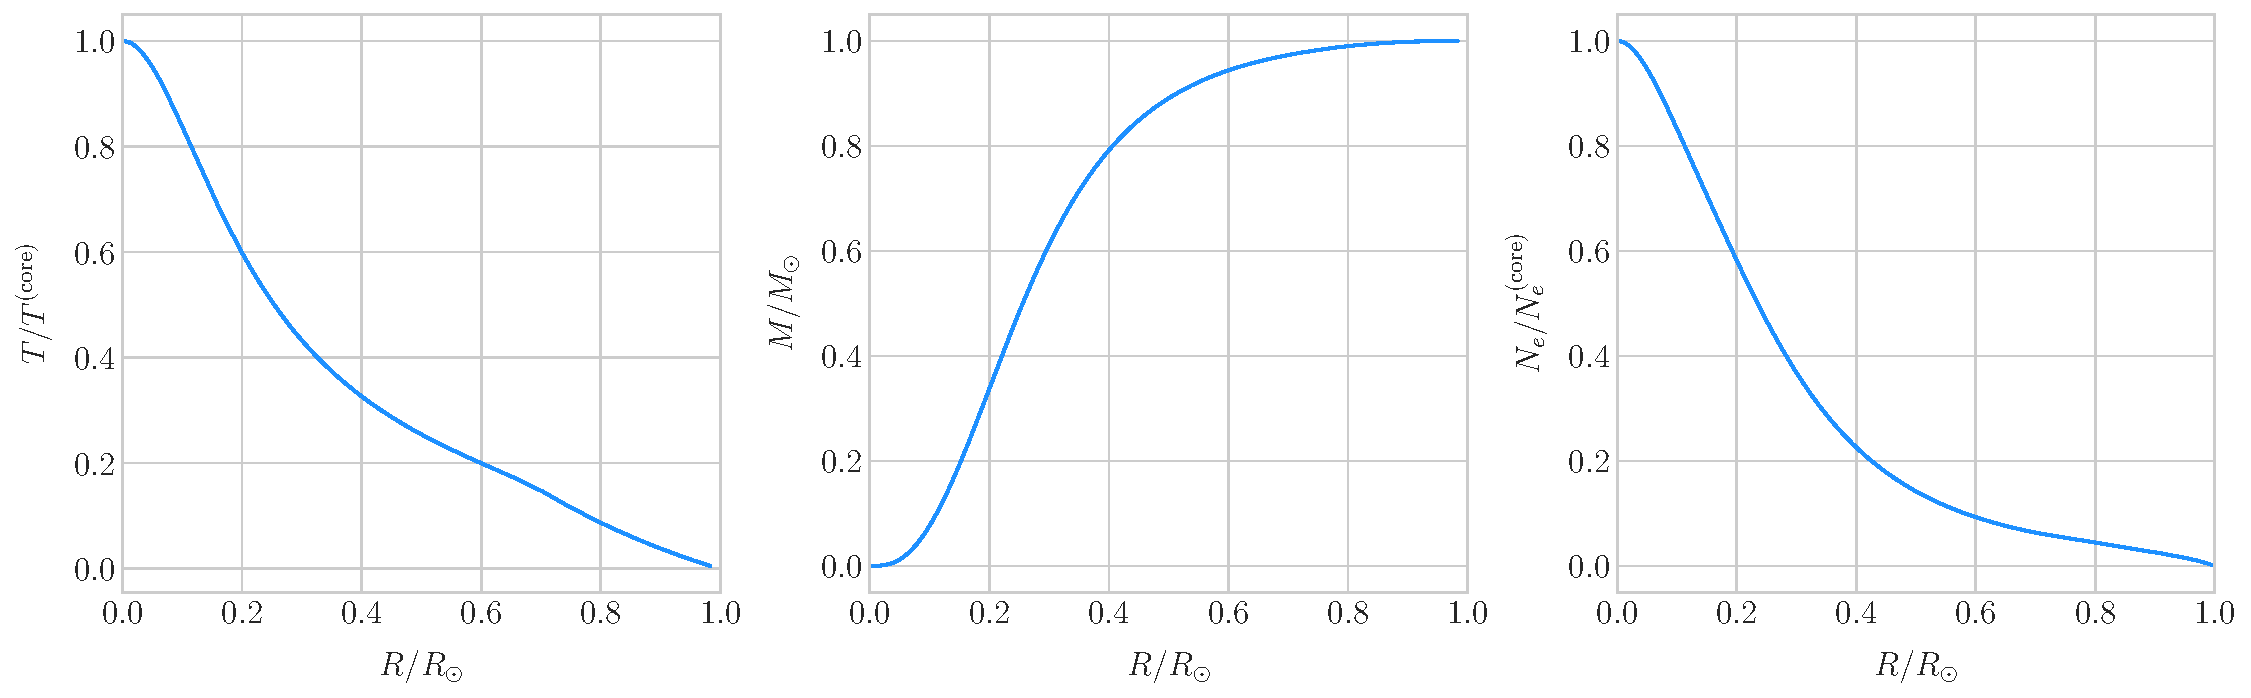
\includegraphics[width=1\linewidth]{Images/DM_Analysis/ssm_params.pdf}
	\caption[Input solar parameters used in the capture rate computation as a function of the solar radius.]{Input solar parameters used in the capture rate computation as a function of the solar radius, from left to right: temperature (with respect to the temperature at the core), mass (in solar masses) and electron number density (with respect to the electron density at the core). All quantities shown correspond to the standard solar model BS2005-OP \cite{Bahcall2004}.}
	\label{fig:ssm_params}
\end{figure}

Finally, if one assumes the \gls{dm} halo velocity distribution in the galactic rest frame to be a Maxwell-Boltzmann distribution, one can write the halo velocity distribution for an observer moving at the speed of the Sun with respect to the \gls{dm} rest frame as:
\begin{equation}\label{2.12}
	f_{v_{\odot}}(u_{\chi}) = \sqrt{\frac{3}{2\pi}} \frac{u_{\chi}}{v_{\odot} v_{d}} \left(\mathrm{e}^{-\frac{3(u_{\chi}-v_{\odot})^{2}}{2v_{d}^{2}}}-\mathrm{e}^{-\frac{3(u_{\chi}+v_{\odot})^{2}}{2v_{d}^{2}}}\right),
\end{equation}
where:
\begin{equation}\label{2.13}
	\omega^{2}(r) = u_{\chi}^{2} + v_{e}^{2}(r),
\end{equation}
is the \gls{dm} velocity squared, $v_{\odot}$ the relative velocity of the Sun from the \gls{dm} rest frame and $v_{d} \simeq \sqrt{3/2} v_{\odot}$ the velocity dispersion.

For the case of strong scattering cross sections, Eq. (\ref{2.5}) ceases to be valid, as it escalates indefinitely with the cross section. In that limit, the capture rate saturates to the case where the probability of interaction is equal to one, which can be written as \cite{Gould1987a}:
\begin{equation}\label{2.14}
	C_{\odot}^{\mathrm{geom}} = \pi R_{\odot}^{2} \left(\frac{\rho_{\chi}}{m_{\chi}}\right) \expval{v} \left(1+\frac{3}{2}\frac{v_{e}^{2}(R_{\odot})}{v_{d}^{2}}\right) \xi(v_{\odot}, v_{d}),
\end{equation}
where $\expval{v} = \sqrt{8/3\pi} v_{d}$ is the mean velocity in the \gls{dm} rest frame and the factor $\xi(v_{\odot}, v_{d})$ accounts for the suppression due to the motion of the Sun:
\begin{equation}\label{2.15}
	\xi(v_{\odot}, v_{d}) = \frac{v_{d}^{2}\mathrm{e}^{-\frac{3v_{\odot}^{2}}{2v_{d}^{2}}}+\sqrt{\frac{\pi}{6}}\frac{v_{d}}{v_{\odot}}\left(v_{d}^{2}+3v_{e}^{2}(R_{\odot})+3v_{\odot}^{2}\right)\mathrm{Erf}\left(\sqrt{\frac{3}{2}}\frac{v_{\odot}}{v_{d}}\right)}{2v_{d}^{2}+3v_{e}^{2}(R_{\odot})}.
\end{equation}

Having these into account, one can write the total capture rate as a combination of both contributions, allowing a smooth transition between the two, as \cite{Bernal2012}:
\begin{equation}\label{2.16}
	C_{\odot} = C_{\odot}^{\mathrm{weak}} \left(1-\mathrm{e}^{C_{\odot}^{\mathrm{geom}}/C_{\odot}^{\mathrm{weak}}}\right).
\end{equation}

\begin{figure}[t]
	\centering
	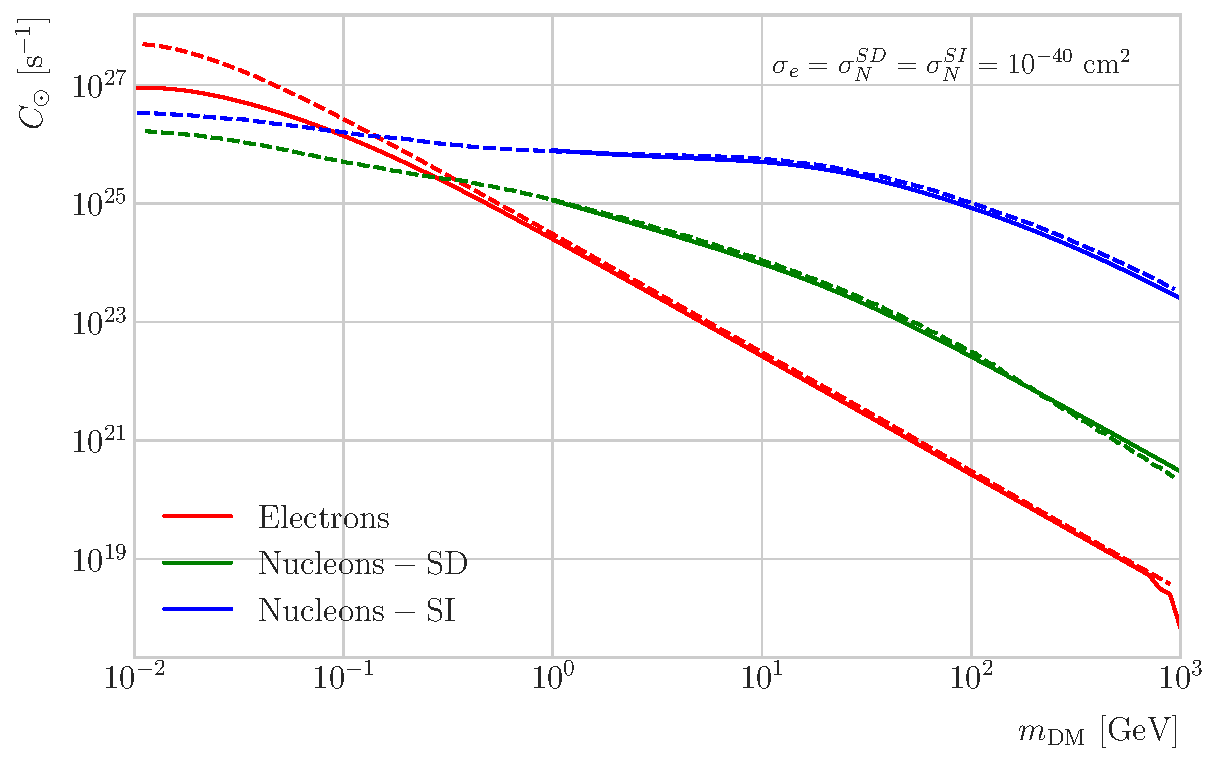
\includegraphics[width=0.9\linewidth]{Images/DM_Analysis/capture_rates.pdf}
	\caption[Capture rates as a function of the \gls{dm} mass for the \gls{dm}-electron interactions, \gls{sd} \gls{dm}-nucleons interactions, and \gls{si} \gls{dm}-nucleons interactions.]{Capture rates as a function of the \gls{dm} mass for the \gls{dm}-electron interactions (red lines), \gls{sd} \gls{dm}-nucleons interactions (green lines), and \gls{si} \gls{dm}-nucleons interactions (blue lines). Solid lines represent the values computed in this work while the dashed lines are the one given in Ref. \cite{Palomares2017}. All the rates are shown for a choice of scattering cross section of $\sigma_{i} = 10^{-40} \ \mathrm{cm}^{2}$.}
	\label{fig:capture_rates}
\end{figure}

I computed the capture rate from Eq. (\ref{2.16}) in the case of interactions with electrons. To do so, I used the standard solar model BS2005-OP \cite{Bahcall2004}. Fig. \ref{fig:ssm_params} shows the three parameters from the solar model that are needed for the computation, the solar temperature (left panel), mass (central panel) and electron density (right panel) profiles.

For the case of the interactions off nuclei, the computations are more convoluted as one needs to add up the contributions of the different most abundant nuclei in the Sun. Also, in contrast to the electron scenario where the form factor is trivially $|F_{e}(q)|^{2} = 1$, for any nucleus $i$ one would need to consider some appropriate nuclear density distribution (either a Gaussian approximation, a Woods-Saxon distribution, etc) which would complicate the calculations even further.

That is the reason why, at this stage of the study, I decided to take an alternative approach to the computation of the \gls{dm}-nucleus capture rates. I used the \texttt{DarkSUSY} software, that allows us to compute these quantities performing a full numerical integration over the momentum transfer of the form factors \cite{Bringmann2018}. The default standard solar model used by \texttt{DarkSUSY} is BP2000\footnote{This is what they say in their manual, but I fear it is somewhat outdated. It appears to me this model is relatively old and do not see why they are not using others like \cite{Bahcall2004}. Maybe one can double-check in the code to make sure.} \cite{Bahcall2000}.

In Fig. \ref{fig:capture_rates} I show the results I obtain for the capture rates, for the case of interactions off electrons (red solid line), \gls{sd} (green solid line) and \gls{si} (blue solid line) interactions of nucleons. In all cases I use a value of the scattering cross sections of $\sigma_{i} = 10^{-40} \ \mathrm{cm}^{2}$. Note here one of the limitations of the \texttt{DarkSUSY} approach, one can not extend the computation below $m_{\mathrm{DM}} = 1 \ \mathrm{GeV}$. Nevertheless, this is not something to worry about in this case, as I will discuss next. As a comparison, I added also the values computed in Ref. \cite{Palomares2017} (same color scheme, dashed lines). One can see there is good agreement between these and the \texttt{DarkSUSY} computation of the \gls{sd} and \gls{si} interactions for $m_{\mathrm{DM}} \geq 1 \ \mathrm{GeV}$. In this regime their computations also matches quite well the results for the electron capture rate. However, these start to differ significantly below $m_{\mathrm{DM}} = 1 \ \mathrm{GeV}$, being their estimate up to a factor of $5$ bigger than ours for low masses. This could be due to the use of a different solar model in the calculation.

Let me comment briefly about the assumption I made before about not including an evaporation term in the Boltzmann equation. If I include this term in the equation, which is proportional to the number of \gls{dm} particles, the equilibrium solution takes the form:
\begin{equation}\label{2.17}
	N_{DM}^{eq} = \sqrt{\frac{C_{\odot}}{A_{\odot}}} \frac{1}{\kappa + \frac{1}{2} E_{\odot} \tau_{eq}},
\end{equation}
where $E_{\odot}$ is the total evaporation rate, $\tau_{eq}$ is the equilibrium time in the absence of evaporation:
\begin{equation}\label{2.18}
	\tau_{eq} = \frac{1}{\sqrt{C_{\odot} A_{\odot}}},
\end{equation}
and $\kappa$ is defined as:
\begin{equation}\label{2.19}
	\kappa \equiv \sqrt{1+\left(\frac{E_{\odot}\tau_{eq}}{2}\right)^{2}}.
\end{equation}

Now, it is easy to proof that in the case evaporation dominates $\kappa \gg 1$ and therefore:
\begin{equation}\label{2.20}
	N_{DM}^{eq} \simeq \frac{C_{\odot}}{E_{\odot}}.
\end{equation}
In contrast, if evaporation is irrelevant $\kappa \simeq 1$ and one recovers Eq. (\ref{2.2}).

In this way, one can define the evaporation mass as the mass for which the number of \gls{dm} particles in equilibrium approaches Eq. (\ref{2.20}) at $10 \%$ level:
\begin{equation}\label{2.21}
	\left| N_{DM}^{eq}(m_{\mathrm{evap}}) - \frac{C_{\odot}(m_{\mathrm{evap}})}{E_{\odot}(m_{\mathrm{evap}})} \right| = 0.1 N_{DM}^{eq}(m_{\mathrm{evap}}).
\end{equation}
This can be regarded as the minimum testable mass one can reach using the annihilation products of the \gls{dm} in the Sun.

It was reported in Ref. \cite{Palomares2017} that, in the case of both \gls{sd} and \gls{si} \gls{dm} interactions off nuclei, this value ranges from $2$ to $4 \ \mathrm{GeV}$ depending on the specific scattering cross section value, compatible with the usual assumptions in the literature. What is interesting is the case of the electron capture. It was found that, when one applies a cutoff in the velocity distribution of the \gls{dm} trapped in the Sun slightly below the escape velocity, the evaporation mass for the \gls{dm}-electron interaction decreases remarkably. For a moderate choice of $v_{c}(r) = 0.9 v_{e}(r)$ one gets an evaporation mass of around $200$ to $600 \ \mathrm{MeV}$. This possibility opens a region of the parameter space that could be tested with the next generation of neutrino detectors.

\section{Example: Kaluza-Klein Dark Matter}
\label{sec:dm_analysis_kk_dm}

Even though there are plenty of \gls{bsm} theories which provide viable \gls{dm} candidates, the Kaluza-Klein (\gls{kk}) type of models \cite{Kaluza1921, Klein1926} within the universal extra dimensions (\gls{ued}) paradigm naturally predict the existence of a massive, stable particle that can play the role of the \gls{dm}. In the \gls{ued} scenario all the \gls{sm} fields can propagate in one or more compact extra dimensions \cite{Appelquist2000}, as opposed to the idea of brane worlds \cite{Arkani-Hamed1998, Randall1999}, where just gravity can propagate in the bulk while \gls{sm} particles live at fixed points.

Furthermore, in \gls{ued} there is no violation of the translational invariance along the extra dimensions, thus leading to degenerate \gls{kk} modes masses  and also the conservation of the \gls{kk} number in the effective four dimensional theory. At loop level, radiative corrections and boundary terms shift the masses of the \gls{kk} modes and break \gls{kk} number conservation into a \gls{kk} parity. As a result, this theory only contains interactions between an even number of odd \gls{kk} modes, and therefore the lightest among the first \gls{kk} excitations will be stable. This particle is usually denoted as the lightest Kaluza-Klein particle (\gls{lkp}) and its mass is proportional to $1/R$, being $R$ the size of the extra dimension.

\begin{figure}
	\centering
	\begin{subfigure}{0.4\textwidth}
		\centering
		\tikz{
			\begin{feynman}
				% left side: for i1 -- a -- b -- f1
				\vertex                         (i1) {\(B^{1}\)};
				\vertex [below right=2cm of i1] (a);
				\vertex [below=1.5cm of a]      (b);
				\vertex [below left=1.5cm of b] (i2){\(B^{1}\)};

				% right side: i2(e+) and f2(e-)
				\vertex [right=3cm of i1]       (f1) {\(f\)};
				\vertex [right=3cm of i2]       (f2) {\(\bar{f}\)};


				\diagram* {
					% left side
					(i1) -- [boson] (a),% e-
					(a) -- [anti fermion, edge label'=\(f^{1}\)](b),
					(b) -- [anti fermion](f2),% e+
					
					% cross-overs at the right side
					(i2) -- [boson] (b),
					(a) -- [fermion] (f1)
				};

			\end{feynman}
		}
	\end{subfigure}
	\begin{subfigure}{0.4\textwidth}
		\centering
		\tikz{
			\begin{feynman}
				% left side: for i1 -- a -- b -- f1
				\vertex                         (i1) {\(B^{1}\)};
				\vertex [below right=2cm of i1] (a);
				\vertex [below=1.5cm of a]      (b);
				\vertex [below left=1.5cm of b] (i2){\(B^{1}\)};

				% right side: i2(e+) and f2(e-)
				\vertex [right=3cm of i1]       (f1) {\(f\)};
				\vertex [right=3cm of i2]       (f2) {\(\bar{f}\)};


				\diagram* {
					% left side
					(i1) -- [boson] (b),% e-
					(a) -- [anti fermion, edge label=\(f^{1}\)](b),
					(b) -- [anti fermion](f2),% e+
					
					% cross-overs at the right side
					(i2) -- [boson] (a),
					(a) -- [fermion] (f1)
				};

			\end{feynman}
		}
	\end{subfigure}
	\caption{Feynman diagrams for $B^{1}$$B^{1}$ annihilation into \gls{sm} fermions.}
	\label{fig:lkp_diagrams_fermion}
\end{figure}

\begin{figure}
	\centering
	\begin{subfigure}{0.25\textwidth}
		\centering
		\tikz{
			\begin{feynman}
				% left side: for i1 -- a -- b -- f1
				\vertex                         (i1) {\(B^{1}\)};
				\vertex [below right=2cm of i1] (a);
				\vertex [below=1.5cm of a]      (b);
				\vertex [below left=1.5cm of b] (i2){\(B^{1}\)};

				% right side: i2(e+) and f2(e-)
				\vertex [right=3cm of i1]       (f1) {\(\phi\)};
				\vertex [right=3cm of i2]       (f2) {\(\phi^{*}\)};


				\diagram* {
					% left side
					(i1) -- [boson] (a),% e-
					(a) -- [scalar, edge label'=\(\phi^{1}\)](b),
					(b) -- [scalar](f2),% e+
					
					% cross-overs at the right side
					(i2) -- [boson] (b),
					(a) -- [scalar] (f1)
				};

			\end{feynman}
		}
	\end{subfigure}
	\begin{subfigure}{0.25\textwidth}
		\centering
		\tikz{
			\begin{feynman}
				% left side: for i1 -- a -- b -- f1
				\vertex                         (i1) {\(B^{1}\)};
				\vertex [below right=2cm of i1] (a);
				\vertex [below=1.5cm of a]      (b);
				\vertex [below left=1.5cm of b] (i2){\(B^{1}\)};

				% right side: i2(e+) and f2(e-)
				\vertex [right=3cm of i1]       (f1) {\(\phi\)};
				\vertex [right=3cm of i2]       (f2) {\(\phi^{*}\)};


				\diagram* {
					% left side
					(i1) -- [boson] (b),% e-
					(a) -- [scalar, edge label=\(\phi^{1}\)](b),
					(b) -- [scalar](f2),% e+
					
					% cross-overs at the right side
					(i2) -- [boson] (a),
					(a) -- [scalar] (f1)
				};

			\end{feynman}
		}
	\end{subfigure}
	\begin{subfigure}{0.25\textwidth}
		\centering
		\tikz{
			\begin{feynman}
				% left side: for i1 -- a -- b -- f1
				\vertex                         (i1) {\(B^{1}\)};
				\vertex [below right=2cm of i1] (a);
				\vertex [below left=1.5cm of a] (i2){\(B^{1}\)};

				% right side: i2(e+) and f2(e-)
				\vertex [right=3cm of i1]       (f1) {\(\phi\)};
				\vertex [right=3cm of i2]       (f2) {\(\phi^{*}\)};


				\diagram* {
					% left side
					(i1) -- [boson] (a),% e-
					(a) -- [scalar](f2),% e+
					
					% cross-overs at the right side
					(i2) -- [boson] (a),
					(a) -- [scalar] (f1)
				};

			\end{feynman}
		}
	\end{subfigure}
	\caption{Feynman diagrams for $B^{1}$$B^{1}$ annihilation into a Higgs boson pair.}
	\label{fig:lkp_diagrams_scalar}
\end{figure}

A viable \gls{dm} candidate needs to be electrically neutral and non-baryonic, therefore good candidates among the first Kaluza-Klein excitations would be the \gls{kk} neutral gauge bosons and the \gls{kk} neutrinos \cite{Servant2002}. Another possible candidate is the first \gls{kk} excitation of the graviton, which receives negligible radiative contributions to its mass and therefore has a mass almost equal to $1/R$. However, it has been shown that the lightest eigenstate from the mixing of the gauge mass states $\left(B^{1},~ W_{3}^{1}\right)$ would be lighter, as these receive negative radiate corrections \cite{Cheng2002}. It is also understood that, when these corrections become sizeable, the eigenstates become approximately pure $B^{1}$ and $W_{3}^{1}$ states, as the Weinberg mixing angle grows small with the \gls{kk} number \cite{Cheng2002}. In that case, the \gls{lkp} can be well-approximated as being entirely $B^{1}$.

\begin{figure}[t]
	\centering
	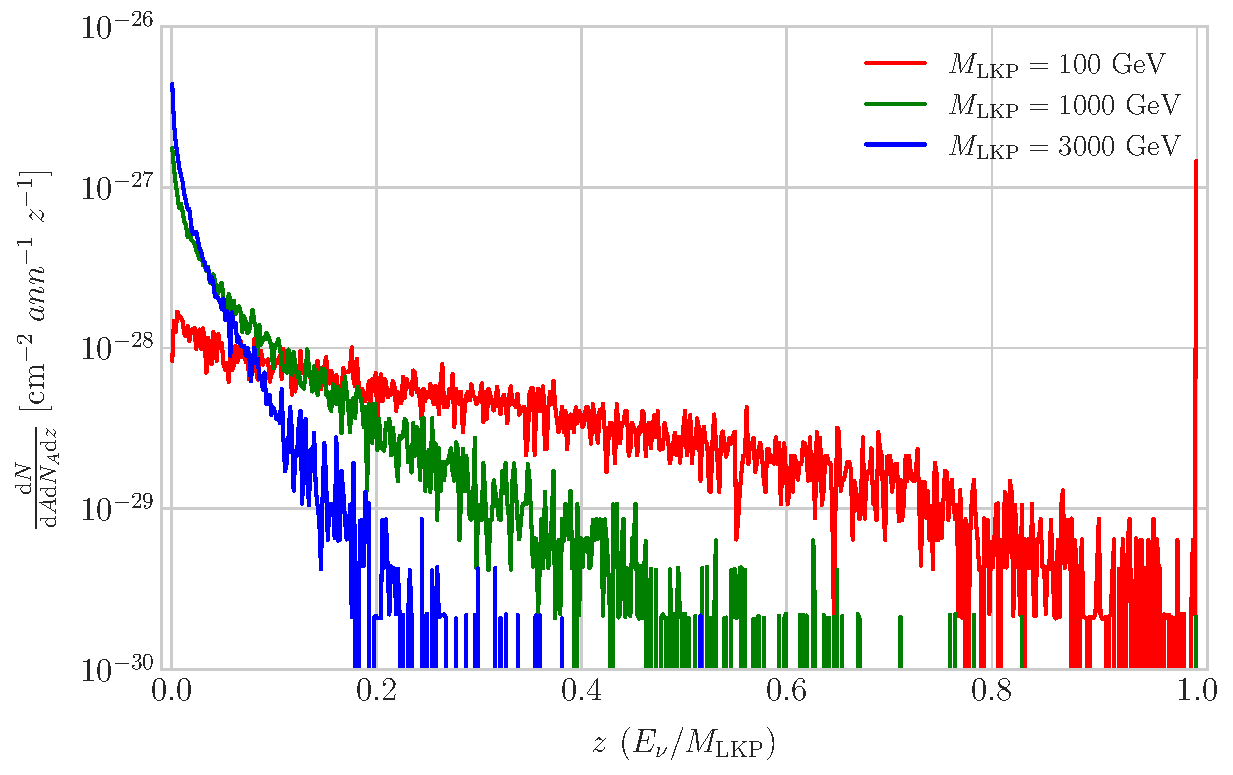
\includegraphics[width=0.9\linewidth]{Images/DM_Analysis/KK_nu_flux}
	\caption[Computed spectra of muon neutrinos at the \gls{dune} \gls{fd} site from $B^{1}$ annihilations in the Sun for various values of $M_{\mathrm{LKP}}$.]{Computed spectra of muon neutrinos at the \gls{dune} \gls{fd} site from $B^{1}$ annihilations in the Sun for three different values of $M_{\mathrm{LKP}}$, plotted in relative energy units for legibility.}
	\label{fig:KK_nu_flux}
\end{figure}

To estimate the sensitivity of \gls{dune} to this particular \gls{dm} model, I first need to compute the neutrino flux produced by the annihilations of the \gls{lkp} in the core of the Sun, taking into account their propagation in the solar medium, as well as neutrino oscillations.  To this end I use \texttt{WimpSim} \cite{Blennow2007, WimpSim} to generate $10^{6}$ annihilation events in the Sun over a time span of four years, and propagate them to the \gls{dune} \gls{fd} location (44$^{\circ} $ 20' N, 103$^{\circ} $ 45' W), for different values of $M_{\mathrm{LKP}}$. The different Feynman diagrams for the annihilation of the $B^{1}$ into a pair of \gls{sm} fermions and scalars are shown in Figs. \ref{fig:lkp_diagrams_scalar} and \ref{fig:lkp_diagrams_scalar}. The relative annihilation fractions of the $B^{1}$ used by \texttt{WimpSim} can be found in Ref. \cite{Hooper2007}.

In Fig. \ref{fig:KK_nu_flux} I show the obtained muon neutrino spectra arriving to the detector from \gls{lkp} annihilations in the Sun, per unit area and per annihilation, plotted in relative energy units for different values of the \gls{lkp} mass. As one could expect the spectra get steeper the higher is the mass, due to the absorption of high-energy neutrinos in the solar medium. Also, one can see  the peak at $z=1$ due to the direct annihilation into neutrinos $B^{1} B^{1} \rightarrow \nu \bar{\nu}$.

Now, one can estimate the sensitivity of \gls{dune} to this particular model by using the method I previously discussed. I use the optimistic estimation of the background efficiency in Eq. (\ref{4.3}) to get an upper bound of the sensitivity. Using it, one can directly compute the number of expected background events to be $N_{B} = 0.11$ for an exposure of $400 \ \mathrm{kT}  \ \mathrm{yr}$. Then, Eq. (\ref{4.5}) give us a value of $N_{S}^{90} = 2.20$ for the $90\%$ exclusion number of expected signal events. Thanks to the cross sections generated with \texttt{NuWro} and the computed neutrino fluxes from $B^{1}$ annihilations in the Sun, I can estimate the limits on the \gls{sd} and \gls{si} \gls{dm}-nucleus cross section using the relation in Eq. (\ref{2.2}) and the capture rates I obtained from \texttt{DarkSUSY}.

\begin{figure}[t]
	\centering
	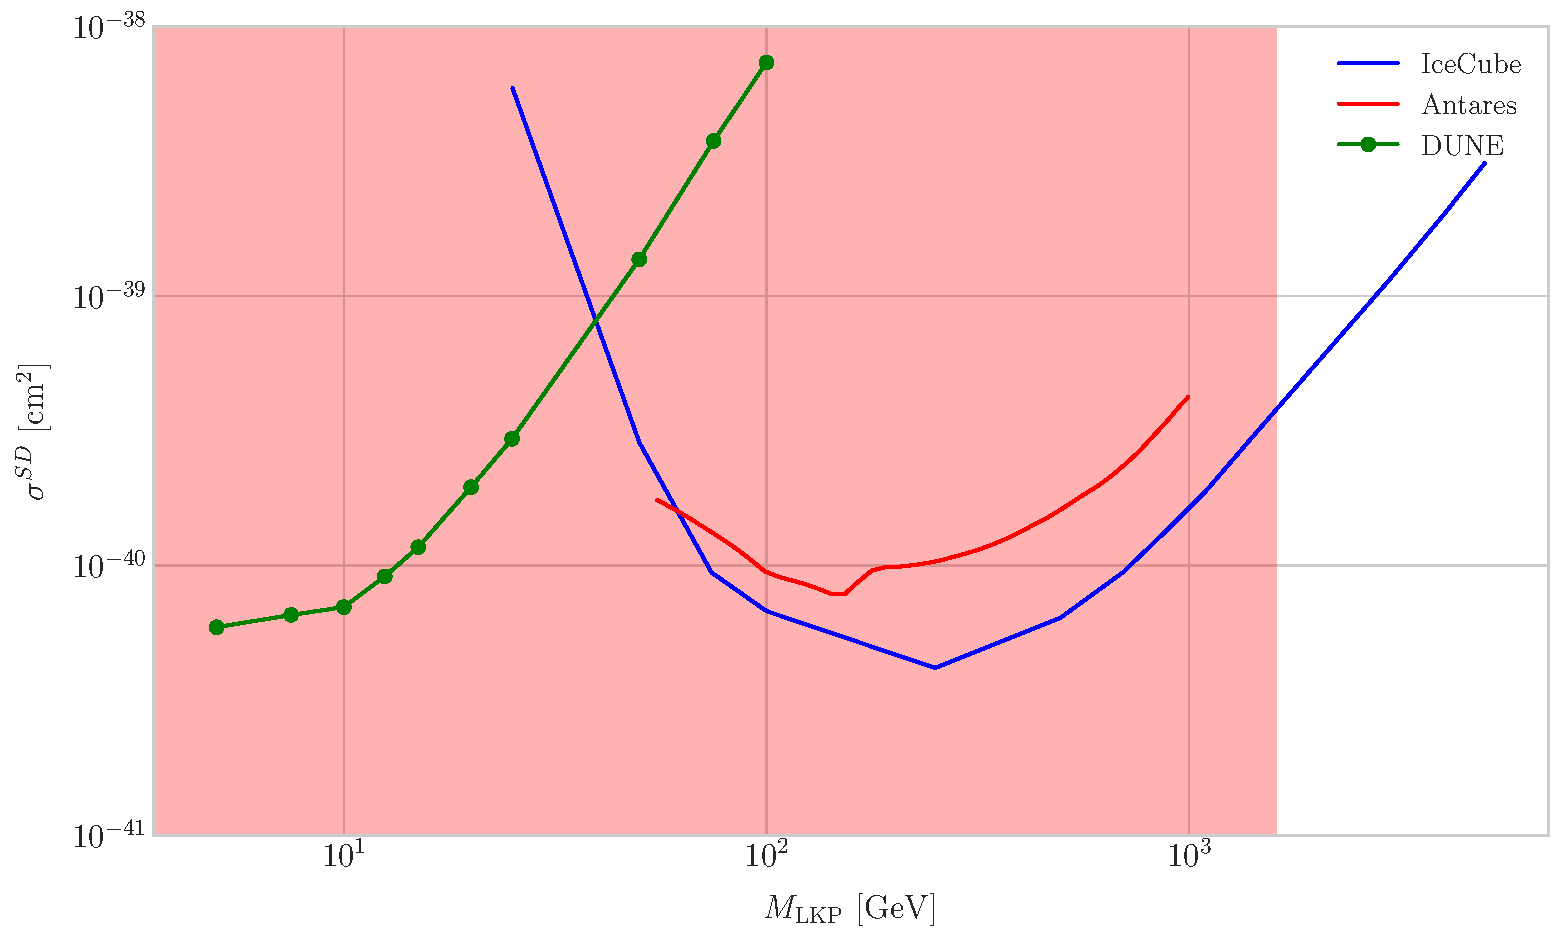
\includegraphics[width=0.9\linewidth]{Images/DM_Analysis/kk_xsection_sd_bounds}
	\caption[Projected 90\% confidence level upper limit for \gls{dune} on the spin-dependent $B^{1}$-proton scattering cross section as a function of $M_{\mathrm{LKP}}$.]{Projected 90\% confidence level upper limit for \gls{dune} (400 kT yr) on the spin-dependent $B^{1}$-proton scattering cross section as a function of $M_{\mathrm{LKP}}$ (green dots). I also show the previous limits from IceCube \cite{Bernadich2019} (blue line) and Antares \cite{Zornoza2012} (red line) on the \gls{lkp} cross section. The shaded area represents the disfavoured region (at 95\% confidence level) on the mass of the \gls{lkp} from \gls{lhc} data \cite{Deutschmann2017}.}
	\label{fig:kk_xsection_sd_bounds}
\end{figure}

In Fig. \ref{fig:kk_xsection_sd_bounds} I show the projected sensitivity for \gls{dune} on the spin-dependent $B^{1}$-proton scattering cross section versus the mass of the \gls{lkp}, for a exposure of $400 \ \mathrm{kT}  \ \mathrm{yr}$ (green dots). I also include the previous results from IceCube \cite{Bernadich2019} (blue line) and Antares \cite{Zornoza2012} (red line). The shaded area represents the disfavoured region from combined searches for \gls{ued} by \gls{atlas} and \gls{cms} \cite{Deutschmann2017}.

From the experimental point of view, this estimation lacked a detailed simulation of the detector response and thus this must be regarded as a mere optimistic sensitivity computation. However, it shows the potential of \gls{dune} to constrain this kind of exotic scenarios, showing the region where it will be in a position to compete with other neutrino telescopes. A more detailed analysis is needed if I am to make a realistic estimation. Even though the region of the parameter space where \gls{dune} would be sensitive to this particular model is quite constrained by collider searches \cite{Deutschmann2017} and other rare decay measurements \cite{Haisch2007, Freitas2008}, it still constitutes an alternative indirect probe.

\section{Example: Leptophilic Dark Matter}
\label{sec:dm_analysis_leptophilic_dm}

In general, the capture rate of \gls{dm} particles by the Sun via interactions with electrons is several orders of magnitude smaller than the capture via \gls{dm}-nucleus scattering. Thus, it would be sub-leading even when nucleon capture is loop suppressed \cite{Kopp2009}. As I showed in Fig. \ref{fig:capture_rates}, the capture rate via scattering off electrons only surpasses the capture rates via \gls{dm}-nucleon interactions for \gls{dm} masses $\lesssim 100 - 500 \ \mathrm{MeV}$.

However, if one considers a model where \gls{dm}-nucleon interactions are forbidden even at loop level, then electron interactions will be the sole contributor to \gls{dm} capture in the Sun. One can describe such scenario where the \gls{dm} particles couple to leptons but not to the quark sector using effective operators.

Assuming that the \gls{dm} particle is a Dirac fermion, the dimension six operators describing the interaction between two \gls{dm} particles and two leptons can be written as:
\begin{equation}\label{7.1}
	\mathcal{L}_{eff} = G \sum_{i} \left(\bar{\chi} \Gamma^{i}_{\chi} \chi\right)\left(\bar{\ell} \Gamma^{i}_{\ell} \ell\right),
\end{equation}
where $G=1/\Lambda^{2}$ is the effective coupling strength, $\Lambda$ the cut-off of the effective field theory and $\ell$ denotes any lepton. In principle, one should consider all the possible Lorentz structures $\Gamma^{i}_{f}$ in order to have a complete set of effective operators.

However, some combinations will induce interactions with nucleons at loop level. As we are specifically interested in interactions which forbid any communication with the quark sector, I will not consider those \cite{Kopp2009}. In addition, some of the effective operators give rise to velocity-suppressed scattering cross sections between \gls{dm} particles and leptons. I will also neglect them, as the suppression goes with the square of the \gls{dm} halo velocity, which in units of the speed of light is $\sim 10^{-6}$.

This way, the only Lorentz tensor structure that do not induce interactions with quarks at loop level and gives a contribution to the scattering cross section that is not velocity-suppressed is the axial-axial interaction. The effective Lagrangian is then given by:
\begin{equation}\label{7.2}
	\mathcal{L}_{eff} = \frac{c_{A}^{\chi} c_{A}^{\ell}}{\Lambda^{2}} \left(\bar{\chi} \gamma^{\mu}\gamma^{5} \chi\right)\left(\bar{\ell} \gamma_{\mu}\gamma^{5} \ell\right),
\end{equation}
where $c_{A}^{\chi}$ and $c_{A}^{\ell}$ are the couplings for the different species. As the \gls{dm} coupling appears as a common factor for any lepton choice, I redefine the corresponding coupling $c_{A}^{\ell}$ to absorb $c_{A}^{\chi}$. Also, for simplicity, I will assume that the couplings between the \gls{dm} particles and the leptons are flavour independent, i.e. I have just two couplings, $c_{A}^{e}$ for charged leptons and $c_{A}^{\nu}$ for neutrinos.

In the case of a scalar \gls{dm} particle, the lowest order effective interaction with leptons happens through a dimension five operator, generating scalar and pseudoscalar interactions. However, the former induces interactions with quarks at two loop level whereas the latter gives a velocity suppressed scattering cross section.

From the effective Lagrangian in Eq. (\ref{7.2}), it can be shown that the axial-axial contribution to the scattering cross section for the fermionic \gls{dm} and a charged lepton is given by:
\begin{equation}\label{7.3}
	\sigma_{\mathrm{DM}-e}^{AA} = 3 \left(c_{A}^{e}\right)^{2} \frac{m_{e}^{2}}{\pi \Lambda^{4}}.
\end{equation}

If the \gls{dm} interacts exclusively with fermions, then the only annihilation channels that will give us measurable neutrino fluxes coming out of the Sun are $\tau^{+}\tau^{-}$ and $\nu\bar{\nu}$. The former channel, already explored previously in the mainstream scenario of the \gls{dm} capture via scattering off nucleons, is open only for $m_{\mathrm{DM}} > m_{\tau} \simeq 1776.86 \pm 0.12 \ \mathrm{MeV}$ \cite{ParticleDataGroup2020}, a mass region where the solar \gls{dm} capture by electrons is at least one order of magnitude smaller than the capture via interactions with nucleons. On the contrary, the latter allows us to explore a region where the capture rate via scattering off electrons dominates over the rest.

One downside of focusing in such low mass range is that it falls bellow the usual limit of $m_{\mathrm{evap}} \sim 4 \ \mathrm{GeV}$ usually explored in the literature. The pretext to explore this region is the result discussed previously reported in Ref. \cite{Palomares2017}, where \gls{dm} evaporation in the Sun for the case of capture via electron scattering could be negligible for masses as low as $m_{\mathrm{evap}} \sim 200 \ \mathrm{MeV}$. This result is quite sensitive to the high velocity tail of the \gls{dm} velocity distribution in equilibrium inside the Sun, and therefore full numerical simulations would be needed to assess the impact of this effect. However, this is out of the scope of this work.

In this case, as I have an specific realisation of the interaction between the \gls{dm} and leptons, I can estimate the relic density of our \gls{dm} for different values of the couplings and the effective field theory scale $\Lambda$. The first step to do so is compute the self-annihilation cross section. Because I consider cold relics, at the freeze-out time our \gls{dm} particles were non-relativistic and so one can expand the annihilation cross section in terms of the relative velocity $v$ between two annihilating \gls{dm} particles as \cite{Beltran2008}:
\begin{equation}\label{7.4}
	\sigma_{ann}^{AA}|v| \approx \frac{1}{2\pi\Lambda^{4}} \sum_{\ell} \left(c_{A}^{\ell}\right)^{2} m_{\chi}^{2} \sqrt{1-\frac{m_{\ell}^{2}}{m_{\chi}^{2}}} \left[\frac{m_{\ell}^{2}}{m_{\chi}^{2}}+\frac{1}{12}\left(2-\frac{m_{\ell}^{2}}{m_{\chi}^{2}}\right)v^{2}\right],
\end{equation}
where the sum includes all the possible lepton final states with mass $m_{\ell}$.

Solving the Boltzmann equation for the evolution of the \gls{dm} density gives as a solution a relic density of:
\begin{equation}\label{7.5}
	\Omega_{\chi} h^{2} \approx \frac{(1.04 \times 10^{9}) x_{F}}{M_{Pl} \sqrt{g_{*}}(a+3b/x_{F})},
\end{equation}
where $x_{F} = m_{\chi}/T_{F}$ being $T_{F}$ the freeze-out temperature, $g_{*}$ the number of relativistic degrees of freedom at freeze-out and $a$ and $b$ the terms in the annihilation cross section expansion $\sigma_{ann} |v| \approx a + b v^{2} + \mathcal{O}(v^{4})$. Using the current best fit for the relic \gls{dm} density $\Omega_{\chi} h^{2} = 0.1198 \pm 0.0012$ \cite{Planck2018} one can use these relations to compute the required effective theory scale $\Lambda$ at which the correct density is achieved for any combinations of $m_{\chi}$ and $c_{A}^{\ell}$.

\begin{figure}[t]
	\centering
	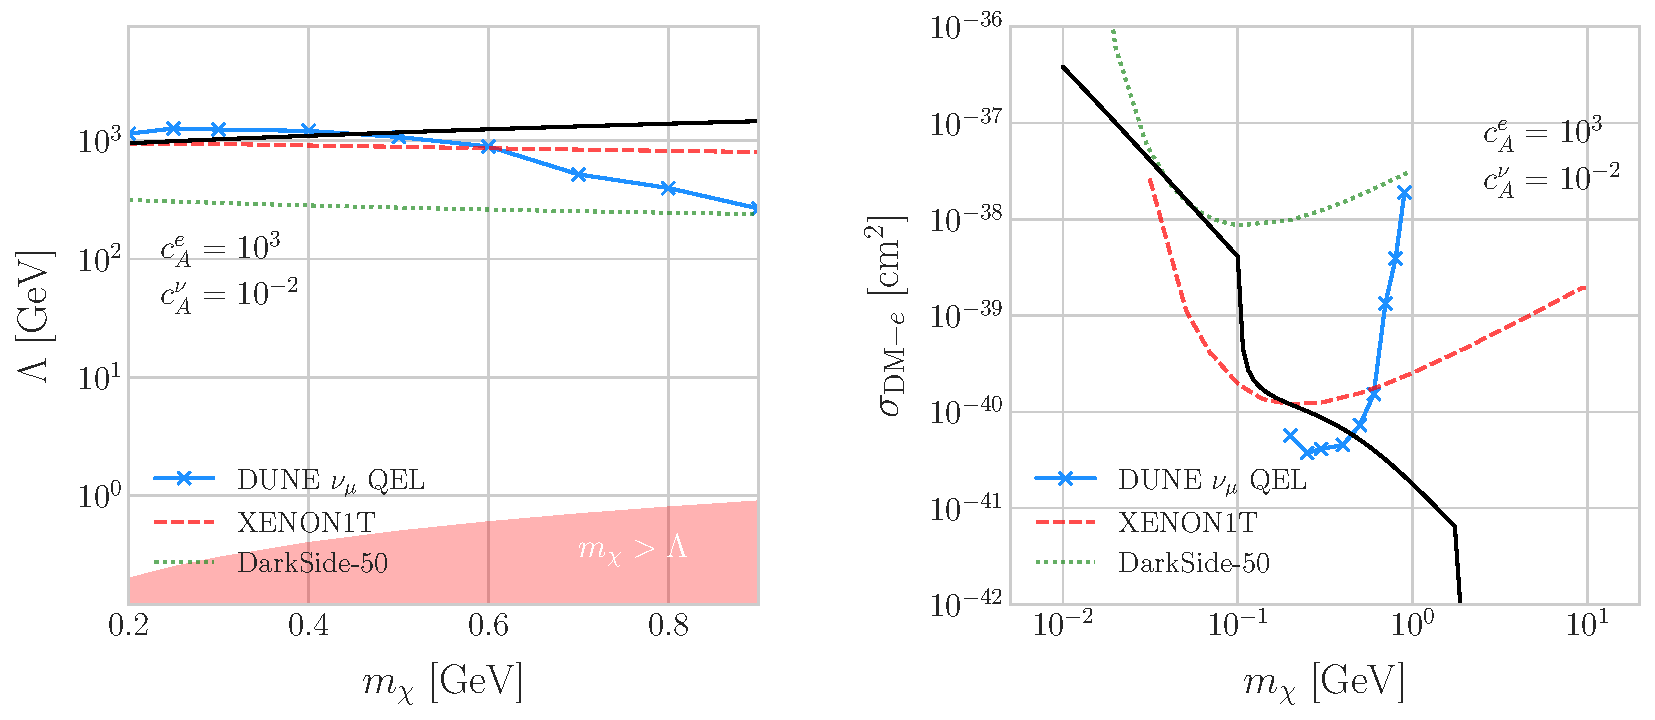
\includegraphics[width=1\linewidth]{Images/DM_Analysis/eft_bounds.pdf}
	\caption[Projected 90\% confidence level sensitivity of \gls{dune} to the scale $\Lambda$ of an \gls{eft} containing only leptophilic \gls{dm} axial-axial interactions.]{Left panel: Projected 90\% confidence level sensitivity of \gls{dune} (400 kT yr) to the scale $\Lambda$ of an \gls{eft} containing only leptophilic \gls{dm} axial-axial interactions (blue line), for the coupling values $c_{A}^{e} = 10^{3}$ and $c_{A}^{\nu} = 10^{-2}$. The black line represents the values for which the correct relic density is achieved. Right panel: Excluded values of $c_{A}^{e}$ as a function of the \gls{dm} mass, for a fixed value $c_{A}^{\nu} = 10^{-2}$. In both cases the corresponding limits from XENON1T \cite{XENON2019} (red), DarkSide-50 \cite{DarkSide2022} (green) and PandaX-II \cite{PandaX-II2021} (magenta) are also shown.}
	\label{fig:eft_bounds}
\end{figure}

As discussed before, in the low \gls{dm} mass region \gls{qe} interactions dominate. Moreover, if I focus on direct annihilation to neutrinos, the energy of the muon neutrino flux is known. This must be equal to the mass of the \gls{dm} particle, $E_{\nu} = m_{\chi}$. That way, now I do not need to use Eq. (\ref{6.6}) in order to estimate the momentum transfer to the remnant nucleus, I can simply take:
\begin{equation}\label{7.6}
	\vec{p}_{N} = \hat{p}_{\nu} m_{\chi} - \vec{p}_{\mu} - \vec{p}_{p}.
\end{equation}

To estimate the signal efficiency and background rejection for this case I use again the \gls{bdt} classifier from \texttt{scikit-learn}, using the same specifications as before. The only difference now is that I add also the reconstructed neutrino energy as one of the features to train the classifier with, because the characteristic monoenergetic flux for each $m_{\chi}$ value will help to distinguish between signal and background events.

In this case, for masses below $\sim 500 \ \mathrm{MeV}$ I obtain a signal efficiency close to unity while keeping a background rejection of $99.9\%$. For bigger values of the mass, the signal efficiency drops significantly if I require to keep the background acceptance under $0.01\%$. However, because this kind of search is dominated by the background, sacrificing the signal acceptance to keep the background rejection to a minimum enhances the reach of the analysis. This way, for \gls{dm} masses of the order of $m_{\chi} \sim 1 \ \mathrm{GeV}$ I end up with efficiencies as low as $1\%$.

Now, estimating the number of background events using Eq. (\ref{6.12}) one can go on and apply Eqs. (\ref{4.5}) and (\ref{4.6}) together with Eq. (\ref{7.3}) to derive the sensitivity of \gls{dune} to this kind of model. Fig. \ref{fig:eft_bounds} (left panel) shows the potential reach of \gls{dune} to constrain the \gls{eft} scale $\Lambda$ of this model containing only leptophilic \gls{dm} axial-axial interactions (blue line), for a choice of couplings $c_{A}^{e} = 10^{3}$ and $c_{A}^{\nu} = 10^{-2}$. I also include the current limits on the \gls{dm}-electron scattering cross section from XENON1T \cite{XENON2019} (dashed red line), DarkSide-50 \cite{DarkSide2022} (dotted green line) and PandaX-II \cite{PandaX-II2021} (dash-dotted magenta line), reworked with Eq. (\ref{7.3}) to show their implications for the \gls{eft} scale. The values of $\Lambda$ for which the correct \gls{dm} relic density value is achieved for each mass are also shown (black line). This tells us that, for that specific choice of couplings, \gls{dune} would be sensitive to \gls{dm} configurations allowed by the relic density constraint up to a mass of $m_{\chi} \sim 400 \ \mathrm{MeV}$.

In Fig. \ref{fig:eft_bounds} (right panel) I show similar limits for the excluded values of $c_{A}^{e}$ as a function of the \gls{dm} mass, for a fixed $c_{A}^{\nu}=10^{-2}$. I do not show the limits for other values of $c_{A}^{\nu}$, as this parameter has little effect on the phenomenology at hand. From this view, one can see that \gls{dune} would be able to offer complementary information to the low energy \gls{dm}-electron interaction searches performed by direct detection experiments, in a slightly higher mass range.

With the present example, although it focuses on a very specific realisation of the \gls{dm} interactions, I show the potential of \gls{dune} to constrain exotic \gls{dm} scenarios. Thanks to its low backgrounds and superb angular resolution, \gls{dune} will be able to help with the searches for dark sectors physics.